\section{Kasutajaliidese disain}
\label{chapters:analysis_interface_design}
MVP funktsionaalsusega (osa \ref{chapters:analysis_requirements}) prototüübi  realiseerimiseks on vaja luua
veebirakenduse kasutajaliidesele järgmised vaated:
\begin{itemize}
    \item Menüüriba
    \item Registreerimise ja sisselogimise vaated
    \item \textit{Dashboard}-vaate
    \item Kasutaja andmete vaade
    \item Ehitusmaterjalide nimekirja vaade
    \item Ehitusmaterjali loomise ja redigeerimise vaade
    \item Kalkulaatori vaade
    \item Kasutajate nimekiri (administraator)
    \item Parameetrite ja lisaandmete vaade (administraator)
\end{itemize}

Mõned vaated on rollispetsiifilised (nt kasutajate nimekirja administraatori vaade), teised on universaalsed - 
kasutajarolli alusel kasutajaliideses otsustatakse, kas näidata (või lubada) midagi kasutajale või mitte.
Igal tegevusel kontrollitakse kasutajaõigusi täiendavalt ka serveriosas enne tegevuse algust.

Kasutajaliidese disaini projekteerimine on teostatud veebipõhise tarkvaraga \textbf{Figma}. Figma võimaldab 
mugaval viisil luua ja redigeerida lehtede visuaalsed prototüübid ja seostada erinevad vaated omavahel. 

Arendatava veebirakenduse kasutajaliidese disain on minimalistlik, aga samas kaasaaegne. Kasutatakse värvilisi ikoone ja värve
elementide kujunduses, et vältida ülemääraselt ametliku mulje tekkimist. Värvitoonid on valitud selliselt, et 
välimus oleks lakooniline ja professionaalne.

Pealehel (\textit{Dasboard}) näidatakse kaardid, mille kaudu kasutajat juhitakse tööriistadele ja 
moodulitele, millele on kasutajal ligipääs. Administraatori ja tavakasutaja \textit{Dashboard}-vaated
on vastavalt erinevad. \textit{Dashboard}-kaartide näide on toodud Joonisel \ref{fig:desing_dashboard_cards}.
\begin{figure}[ht]
    \centering
    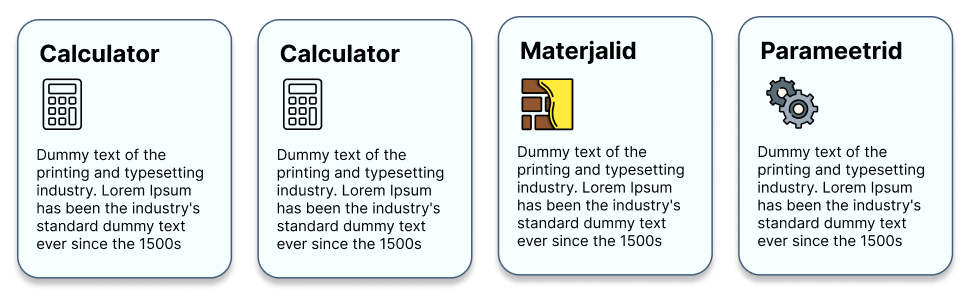
\includegraphics[width=1\textwidth]{figures/analysis/desing_dashboard_cards.png}
    \caption[Pealehe kaartide disaini näide]{\textit{Pealehe kaartide disaini näide}}
    \label{fig:desing_dashboard_cards}
\end{figure}

Kõige keerulisem kasutajaliidese osa on kalkulaatori vaade. Vaade on jaotatud kolmeks loogiliseks osaks:
arvutuse parameetrid, konstruktsiooni kihtide komplekteerimine ja tulemuste graafiline esitamine. 
Kalkulaatori töövoog on esitatud Joonisel \ref{fig:desing_workflow}.
\begin{figure}[ht]
    \centering
    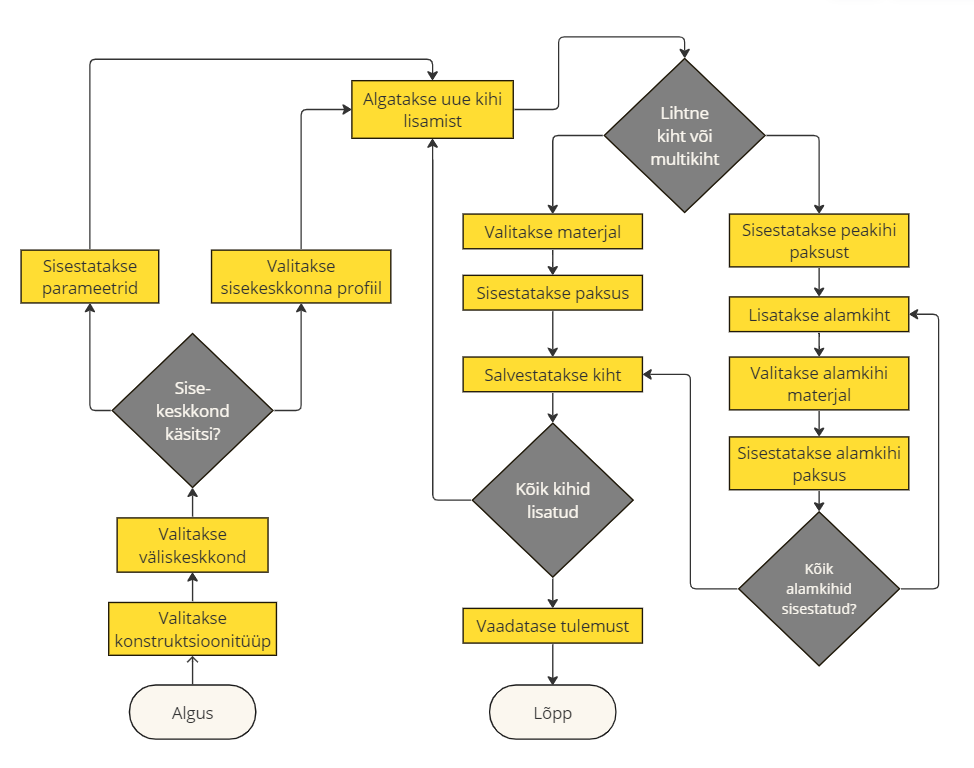
\includegraphics[width=1\textwidth]{figures/analysis/desing_workflow.png}
    \caption[Arvutuse kasutaja töövoog]{\textit{Arvutuse kasutaja töövoog}}
    \label{fig:desing_workflow}
\end{figure}

Parameetrite plokk on esimene, millega peab kasutaja tegelema 
- valitakse arvutuse parameetrid: konstruktsiooni tüüp, väliskeskkond. Samuti valitakse, kas 
sisekeskkonna parameetrid sisestatakse käsitsi või arvutatakse automaatselt välja kasutades 
Eesti elamute sisekliima mudelit. Esimesel juhul kasutajale näidatakse väljad temperatuuri ja 
niiskuse sisestamiseks, teisel juhul näidatakse valiklist sisekeskkonna profiilidega (EN ISO 13788 kohase
klassifikatsiooni järgi).  Samuti selles plokis on esitatud ka arvutuse üldised arvulised tulemused -
konstruktsiooni summaarne soojusjuhtivus (U-arv) ja veeaurutakistus. Parameetrite ploki disain
on näidatud Joonisel \ref{fig:design_calc_parameters}.
\begin{figure}[ht]
    \centering
    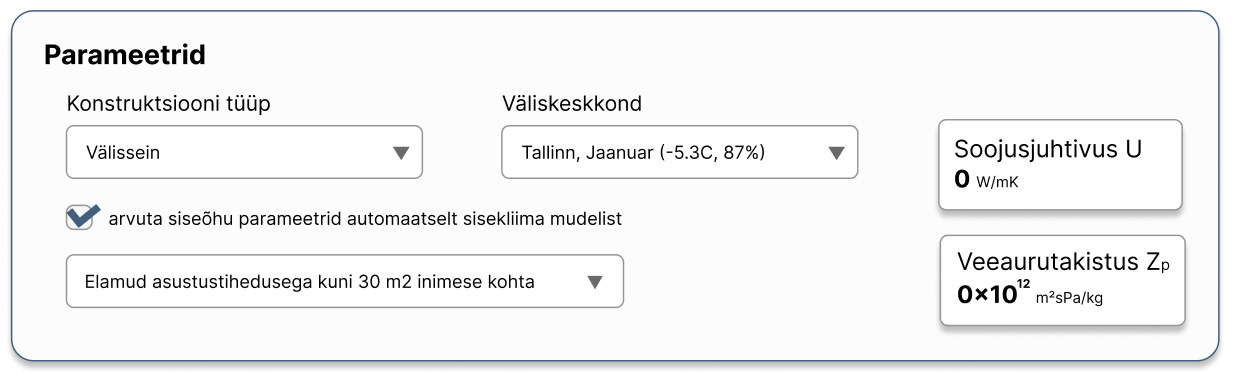
\includegraphics[width=1\textwidth]{figures/analysis/desing_calc_parameters.png}
    \caption[Parameetrite ploki disain]{\textit{Parameetrite ploki disain}}
    \label{fig:design_calc_parameters}
\end{figure}

Järgmine tegevus, mis peab olema tehtud tulemuste näitamiseks on konstruktsiooni mudeldamine, mis
kujutab ennast erinevatest materjalidest ja erineva paksusega kihtidest nimekirja koostamist.
Kasutaja lisab, muudab või kustutab nimekirjas olevad kihid. Uue kihi lisamiseks vajutab kasutaja
vastavat nuppu, mille järel näidatakse uue kihi parameetrite vormi. Vormist peab kasutaja
valima uue kihi materjal, paksust ning salvestada kiht. Kui uue kihi lisamine (või
olemasoleva kihi redigeerimine) on algatatud, siis uue kihi lisamise nupp on deaktiveeritud, et
suunata kasutajad tegeleda vaid ühe kihiga korraga. Lihtsa (ühest materjalist koosneva) kihi lisamise näide
on toodud Joonisel \ref{fig:design_simple_layer}.
\begin{figure}[ht]
    \centering
    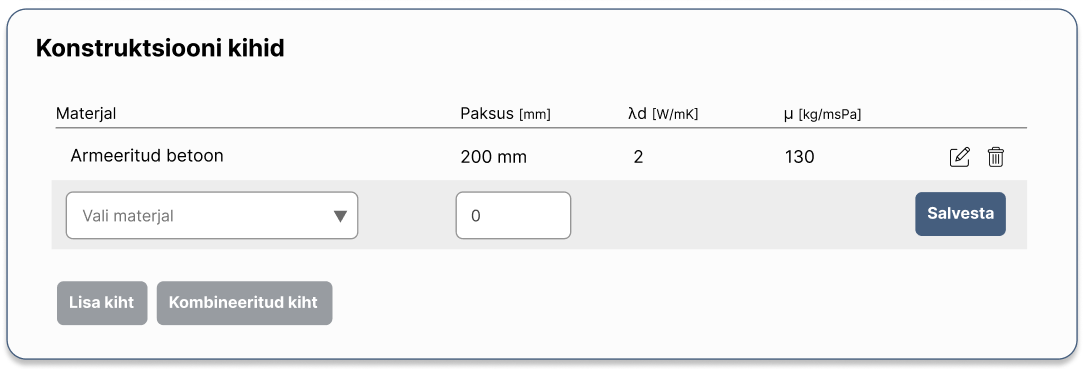
\includegraphics[width=1\textwidth]{figures/analysis/desing_calc_simple_layer.png}
    \caption[Ühest materjalist koosneva kihi lisamine]{\textit{Ühest materjalist koosneva kihi lisamine}}
    \label{fig:design_simple_layer}
\end{figure}

Mittehomogeense (mitmest erinevast materjalist koosneva) kihi lisamine eeldab keerulisemat töövoogu.
Kasutaja kõigepealt peab määrama peakihi paksust (konstruktsiooniga põiki suunas), seejärel lisada 
vajalikku arvu alamkihte ja määrama alamkihtide materjalid ja paksused. Alamkihi paksuseks loetakse 
materjali paksust konstruktsiooniga piki suunas. Kui kõik andmed on valitud, siis uus kiht salvestatakse
vastava nuppu vajutamisega. Mitmest materjalist koosneva kihi lisamise näide on toodud Joonisel \ref{fig:design_simple_layer}.
\begin{figure}[ht]
    \centering
    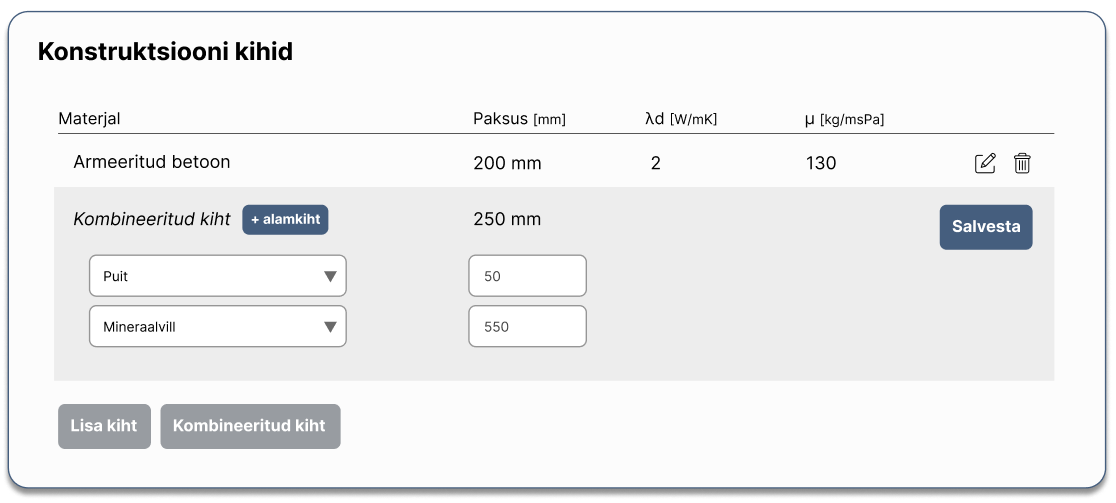
\includegraphics[width=1\textwidth]{figures/analysis/desing_calc_multi_layer.png}
    \caption[Mitmest materjalist koosneva kihi lisamine]{\textit{Mitmest materjalist koosneva kihi lisamine}}
    \label{fig:design_multy_layer}
\end{figure}

Tulemuste esitamiseks tehakse kalkulaatori lehele kaks plokki. Üks neist on mudeldatud konstruktsiooni skemaatiline joonis,
mille peal on näidatud konstruktsiooni kihid paksuste väärtustega ja kasutatud materjaliga. Kihtide tausta värv määratakse
sõltuvalt materjali tüübist (nt betoonid - hall, soojusisolatsioonid - kollane). Tulevikus joonise peale peab lisama 
temperatuuri ja veeauru osarõhkude jaotuse graafikud, kuid prototüübi puhul antud koht on lihtsustatud ja graafikud
on toodud eraldi plokis. Graafikute ehitamiseks kasutatakse valmislahendust, nt Javascript-i põhine teek Graph.js.
Tulemuste plokkide disain on näidatud Joonisel \ref{fig:design_calc_drawing} ja Joonisel \ref{fig:design_calc_graph}..

\begin{figure}[ht]
    \centering
    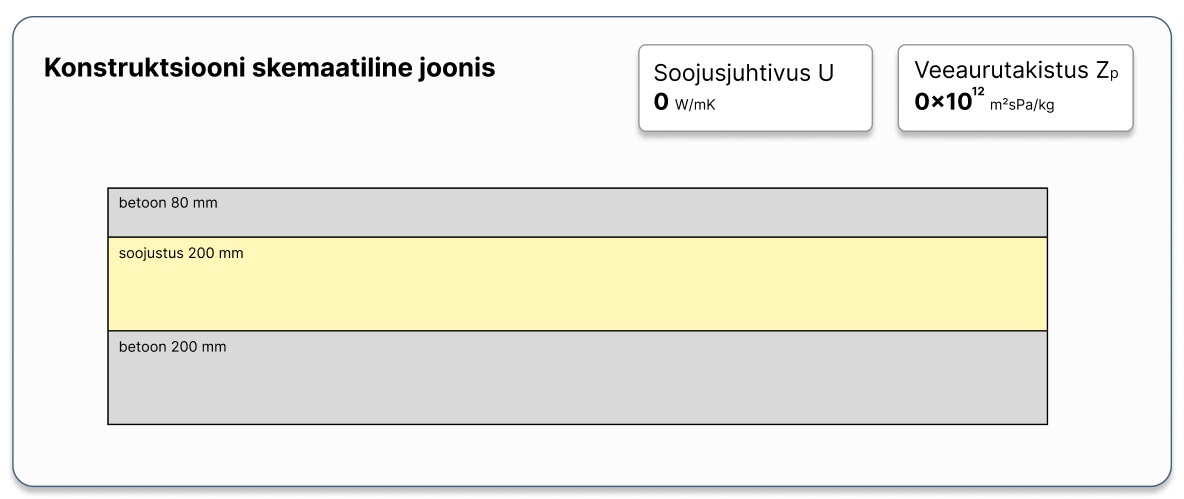
\includegraphics[width=.8\textwidth]{figures/analysis/desing_calc_drawing.png}
    \caption[Konstruktsiooni skemaatiline joonis]{\textit{Konstruktsiooni skemaatiline joonis}}
    \label{fig:design_calc_drawing}
\end{figure}
\begin{figure}[ht]
    \centering
    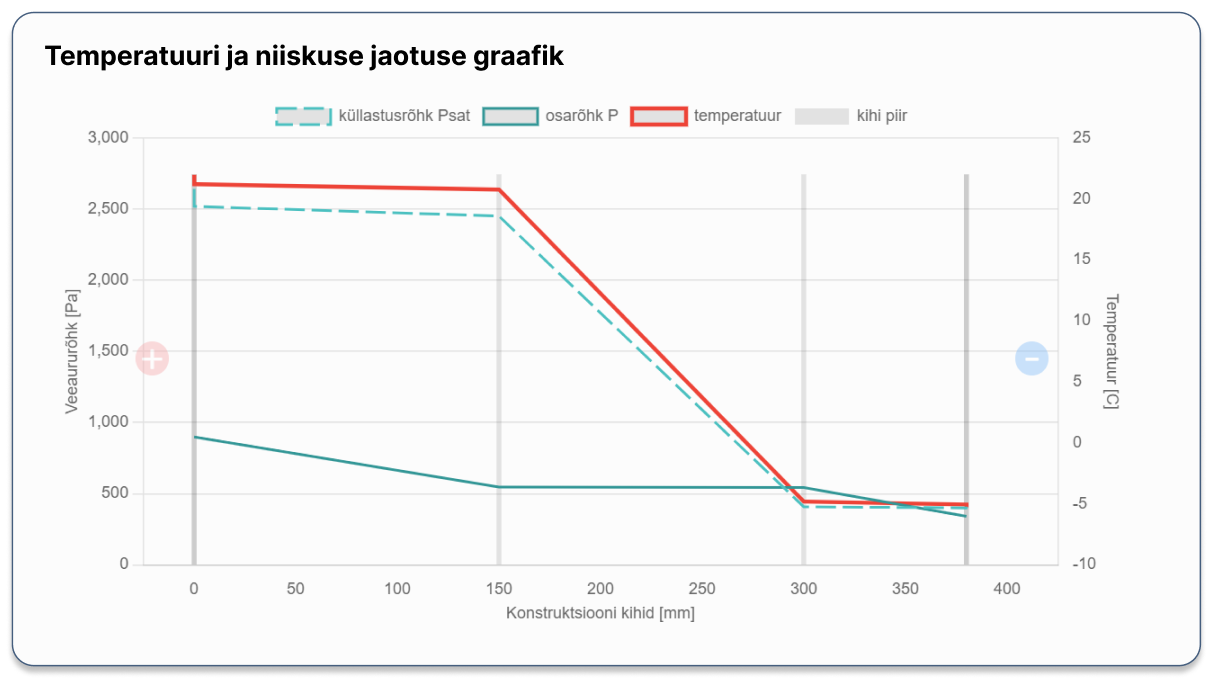
\includegraphics[width=.8\textwidth]{figures/analysis/desing_calc_graph.png}
    \caption[Tulemuste esitamine diagrammil]{\textit{Tulemuste esitamine diagrammil}}
    \label{fig:design_calc_graph}
\end{figure}

Ülejäänud lehed -- ehitusmaterjalid, parameetrid, kasutajad -- kujutavad ennast võrdlemisi lihtsaid CRUD-tüüpi kasutajaliideseid, millistel
keeruline loogika puudub. Kõikide lehtede disaini projektid on esitatud käesoleva töö \colorbox{BurntOrange}{Lisas X}.